\chapter{Safety-critical systems engineering}
\label{chapter:safety}

\section{An introduction to software safety}
  
The trend in systems engineering is toward multi-disciplinary systems. Many of these systems are deployed outside of the standard desktop domain on which programming is typically taught. Such a trend has safety implications: if a piece of software is used to control a hardware system, it may have safety related issues.

For example, consider the following list of applications that have severe safety implications if they fail:

  \begin{itemize}
  \item Computer Aided Dispatch Systems (CAD);
  \item The A320 Airbus Electronic Flight Control System (EFCS);
  \item Biomedical technology, such as pacemakers, and surgical
    robots;
  \item Train protection systems;
  \item Space shuttle;
  \item Automated vehicle braking systems; and
  \item Chemical plant control systems.
\end{itemize}

Such systems have influence well beyond the desktop and an individual user. Software itself cannot harm people -- it is merely an abstraction. However, software, when used to control hardware or other parts of a system (e.g. to make decisions or send orders on behalf of a human), can be a root cause of accidents and incidents.

The systems described above all rely on an integration of different  technologies, and different engineering disciplines.  What is perhaps new to most people in this subject is the reliance on computer systems and software to perform safety critical system functions.


\subsection*{Aims}

The aim of the module on safety engineering is to develop an understanding of the \emph{safety engineering} approach to developing safety-critical systems. Specifically:

\begin{itemize}

  \item We will study accidents to get an idea of how they arise, how
    they are analysed, and what can be done to prevent or mitigate
    accidents.

  \item We will study \emph{safety engineering} processes as the
    pathway to developing and assuring safety critical systems.

  \item We will study the methods of safety analysis and assurance that
    can be applied at all stages of the development process.

\end{itemize}


\section{Why safety engineering?}
\label{sec:safety:safety-engineering}

In the examples above, software is part of a much larger and much
  more complex environment. Running a huge set of tests to show that your software behaves as you expected does not really impact safety a great deal.


In safety-critical systems, testing is a necessary but insufficient means of assuring a safe system.  Remember that testing is about finding faults -- not about showing correctness, and especially not about showing safety.

\emph{Safety and security is not just a software issue.}

  System safety and security involve the hardware that the software is
  running on, the physical devices to which the software is connected
  the people which must operate the systems, and operating procedures
  in force.

\subsection*{Software and its relation to safety}

The following are important themes in safety engineering:

\begin{itemize}

    \item Software is always part of a larger system. 
    
    \item Design faults can exist at various levels:
    
        \begin{itemize}
        
        \item Written requirements do not conform to the actual
          requirements.
           
           \item The specification does not conform to the written 
           requirements.
           
           \item Source code does not conform to the specification.
           
           \item Object code does not match the source code.
        
        \end{itemize}
    
    \item Incorrect requirements are a major cause of accidents.
    
    \item Simple design faults rarely cause accidents \emph{on their
    own}.    

    \item Human error is inevitable:

    \begin{quote}
      ``\emph{Components
    developed over several years are hard to modify. Components which
    have taken several million years to evolve are almost impossible to
    modify.}''
   \end{quote}

\end{itemize}

\subsection*{Is safety equivalent to correctness?}

One initial mistake to make is to think that, provided our software is \emph{correct}, it will be \emph{safe}. This is fallacious thinking.

\begin{quote}
 \textbf{Correctness} -- Correctness alone does guarantee safety.
\end{quote}


Consider a knife. If we assume that it is a good knife and so does not contain any ``faults'' then is it safe? The answer of course relies on how it interacts with its environment, not on whether or not it contains faults. If I do not get my thumb out of the way while cutting, I can harm my thumb. The knife is not safe. But it can still function correctly.

Now, let's turn to a systems engineering example. I can design a braking systems for a car that is 100\% correct, but 0\% safe. My design consists of a braking system with a brake pedal that does nothing. Implementing the design correctly is straightforward: do nothing. But this is surely not safe -- unless the wheels are designed to be square. Again, safety results from how our system interacts with its environment.

This does not imply that we should not also strive for correctness. An incorrectly implemented design is more likely to result in safety concerns than a correctly implemented one.

\subsection*{Is safety equivalent to reliability?}

Is safety then about reliability?

\begin{quote}
  \textbf{Reliability} -- Reliability alone does not guarantee safety.
\end{quote}


Consider a box of matches. An unreliable match --- that is, one that fails to perform its function according to specification --- is far more likely to be ``safe'' than a reliable match.

  \textbf{A common misconception} is that if we just get all of the
  faults out of our system and stop it from failing then all will be
  well and our system will be ``safe''.

  \textbf{Reliability} {\em is the probability that a system will work without failure for a specified period of time in a given environment}. Thus, reliability is about failure.

  Reliability measurements for software are statistical; for example,
  failure intensity (the number of failures observed per unit
  time), the Mean Time Between Failure (MTBF), or failure
    probability gained from testing the computer based part of the
  system.

  The word failure is the key to understanding software reliability.




  \subsection*{Reliability and safety}
  
  A \emph{failure} is a deviation from the specified system behaviour.
 
  A \emph{failure} in a safety critical system is more commonly a
  deviation from the intended behaviour -- which is to be safe -- and
  especially where the deviation can lead to harm or loss.

  In the reliability usage of the word failure, a system may be
  unreliable but still safe, and worse, it may be completely reliable
  but totally unsafe.


  \begin{example}
  Let's consider an example to demonstrate the different between reliability and safety.

  We have already seen that correctness is not the same as safety through the example of the braking system. A similar example can distinguish the difference between reliability and safety. Consider a collection of systems for aircraft.

  If I fly on an aircraft, I want a set of systems that always fly (reliable), while also not crashing (safe). However, I can easily implement an unreliable and safe system: never start the engines. The plan will not be able to move, so will be safe. However, it will not be reliable.

  Now, consider the converse: something that is reliable but unsafe. We can consider the braking system example above: simply design our aircraft system to have no brakes. I can implement the braking system reliability, but the aircraft will not be safe.

While this example is somewhat extreme, it distinguishes the difference between reliability and safety well.
  \end{example}


\section{Safety engineering}
  
\emph{Safety engineering} is the set of processes, methods, and techniques for assuring the system safety. The safety engineering approach is characterised by monitoring safety throughout the product development process -- just like other quality attributes.

The safety engineering process ends by ensuring that there is enough evidence to build a \emph{safety case} to demonstrate that the product is safe. Typically, it is not sufficient just to say (or show) that a large set of tests have been run, or that a design has been carefully crafted. In most countries, regulatory authorities require that a safety case demonstrates that safety concerns have been identified, the system has been designed to consider them, and has been implemented to its design.

\begin{definition}
A \emph{safety case} is a high level argument that is presented to regulatory bodies, or customers, to demonstrate that a system is safe. They are generally built up using all of the evidence gathered during the exploratory, deductive, inductive and design processes.
\end{definition}

There are several phases throughout the system development lifecycle in which safety engineering plays an important role:

\begin{enumerate}

\item {\bf Requirements Analysis and Product Definition} --
  Preliminary Hazard Analysis and other methods are used to determine
  the hazards or potential situations that can cause harm or
  environmental damage. Their potential causes and impacts are listed.

\item {\bf Design and Implementation Phases} -- To guide the design, one typically uses a
  \emph{deductive} approach: one that starts with potential situation of
  harm or injury and works back to design or implementation elements.
  is used. This is typically followed up by an \emph{inductive} approach:
  one that starts from component or subsystem failures.

  During these phases, the system designers and safety engineers work closely to ensure that the design considers the high-risk safety concerns. Systems that must defend against  situations of harm or damage must typically be ultra-reliable or must have sufficient redundancy so that a safety related
  subsystem failure does not lead to a safety related system
  failure. This is the principle of ``Defending in Depth'' against
  potential accidents. We will discuss more about redundancy later in this subject.


\item {\bf Safety Cases} -- Finally, throughout the process, a safety case is constructed, which is used to convinced the customer or regulator authority that the system is safe. That is, all non-trivial hazards are identified and  the design considers these and deals with them appropriately.

\end{enumerate}


\subsubsection*{Concepts in safety engineering}
  
 The terminology used here is consistent with common usage but beware that terminology differs between standards.
 Safety as it concerns us in this subject is chiefly concerned with physical products.

\begin{itemize}

\item  {\bf Platform} --- The largest engineered artifact that contains the software, the physical devices on which the software will run (and which connect people to the system), and the operating procedures.

\item {\bf Unsafe} --- A product is \emph{unsafe} if it causes unacceptable harm; for
  example, in the loss of life, injury or environmental damage.

{\bf Note} an important point here. Considering software in
isolation from the rest of the system does not tell us anything about
its safety or otherwise. When analysing a system for safety the \emph{whole system}, including hardware, other software systems, humans, and the environment, must be considered.

\item \textbf{Safe} --- A product is \emph{safe} if it is not unsafe.

\item {\bf Accident} --- An accident is an unintended event, or more
  typically an unintended sequence of events, leading to harm.

\item {\bf Incident} --- An event that significantly reduces the safety of
  a platform but does not lead to an accident.

  \item {\bf Hazard} ---   a physical situation or state of a platform that can lead to an
    accident.

 \item \textbf{Failure} --- An unintended condition of a system that can lead
  to a hazard.  IEC--61508 states that a \emph{failure} occurs when
  the delivered service deviates from the specified service.

 \item \textbf{Error} --- An unintended state that can lead to a failure.
    
  \item \textbf{Flaw} -- A design defect that can give rise to an error under specific conditions.
    
\item \textbf{Fault} --- An event that occurs when a flaw is activated
  resulting in an error.

\end{itemize}

Note the the definition of \emph{fault} is different in safety engineering than in software testing.

\section{Accidents and safety engineering}

Understanding accidents is key to understanding safety. In this section, we look at accidents and causality.


First, let's consider some pertinent examples of accidents in which software was a primary contributor:

  \begin{description}

    \item[Therac-25]  -- Between June 1985 and January 1987, six people died after receiving more than 100 times the intended radiation dose from Therac-25 radiation therapy machine.

   A commission into the accident concluded that the primary cause of the radiation overdose was from poor software design, not from coding errors.

    \item[A320 Airbus Accidents] -- The Lufthansa A320 accident at
      Warsaw airport, and the Mulhouse-Habsheim Airport accident (discussed in more detail below).

    \item[London Ambulance] -- In October 1992, the failure of the London Ambulance Services' new
      Computer Aided Dispatch (CAD) system resulted in over 30 deaths and
      problems in dealing with life-threatening incidents \cite{finkelstein1996comedy}.

   An investigation concluded that the system was poorly designed and implemented, leading to significant delays in the assigning of ambulances. In some cases, an ambulance took up to 11 hours to arrive.

   An upgrade in July 2006 led to repeated system crashes in July and August, and operators reverted to old pen-and-paper methods for ambulance dispatch. 

   On 8 June 2011, a completely new CAD system, called CommandPoint, was commissioned. On 9 June 2011, the system developed technical problems and operators again had to revert to to old pen-and-paper methods. The London Ambulance Service reverted to the previous CAD system on the same day, and CommandPoint was not re-instated until May 2012.

  \end{description}

\subsection{Case Study: The A320 Airbus}

 The Airbus A320 is a \emph{fly by wire} aircraft, in which the pilot's
  commands are transmitted to the flight control surfaces as electronic
  signals rather than mechanically via cables and pulleys.

  It has been described as a \emph{``network with an aircraft wrapped
  around it''}.  There are about 150 individual computers on board each
  of which must communicate with the others.

  Fly by wire (and drive by wire) are ubiquitous in modern transport systems. They have many advantages over the old mechanical systems \cite{mellor1994cad}:

  \begin{itemize}

  \item Saving in weight.

  \item Enhanced control of the aircraft (e.g. anti-lock brakes).

  \item Simplify retraining.

  \item Simplify maintenance (i.e. software instead of hardware).

  \item The flight engineer is made redundant.

  \item Enhanced safety by creating a protective flight envelope  and
  thereby reducing pilot error.

  \item Marketing advantage.

  \end{itemize}




  \subsubsection*{A320 On Board Systems}

 The A320 has the following on-board systems:

  \begin{itemize}

  \item Electronic Flight Control System ({\bf EFCS}).

  \item Flight Management and Guidance Control system ({\bf FMGC}).

  \item Full Authority Digital Engine Control system ({\bf FADEC}).

  \item Electronic Instruments -- the ``\emph{Glass Cockpit}''.

  \end{itemize}    


  \subsubsection*{Habsheim -- 26 June 1988}

  The intention of the flight was to demonstrate the aircraft's capability at low
  altitude.  It made the first pass slowly at 34ft/10m, flaps extended
  and landing gear down, successfully.  

 
  The second pass was to be done at speed in a \emph{clean}
  configuration (landing gear raised).  The aircraft failed to regain
  altitude, ploughed into a forest at the end of the runway, and
  caught fire, killing 3 of the 130 passengers and injuring 34 others.


  An official investigation of the accident attributed it to the following causes:
\begin{itemize}

\item low fly-over; lower than surrounding obstacles;

\item low speed with engines at flight idle; and

\item late application of ``go around'' thrust.

\end{itemize}

Together with the conclusion that the aircraft was flight worthy and
that no malfunction of the on-board systems contributed to the crash,
the verdict was \emph{pilot error}.

However, an interesting observation has been made by many safety experts that many more aircraft accidents are attributed to pilot error when the pilot dies than when the pilot lives. This indicates a culture of blaming the pilot first, and then seeking their explanation second.

Further to this, many accidents attributed to ``pilot error'' are of the form that: ``the aircraft did X, but the pilots did not notice Y, therefore, they caused the accident''. For example, in some cases, pilots and co-pilots have failed to notice warning lights. This can be considered quite unfair on the pilots: if neither the pilot nor the co-pilot noticed a warning light, surely it could be considered a failure of the warning light system for not being noticeable? If we agree with the quote in Section~\ref{sec:safety:safety-engineering} that human error is inevitable, we should build our systems to consider that humans will make errors, so the system must try to accommodate them.

%------------------------------------------------------------

%%
%%    The Pilot's Version 1
%%



  \subsubsection*{The Pilot's Version}

The pilot actually survived this crash and so his version has been
recorded as well as the official finding. The pilot's versions stated:

\begin{itemize}

\item Company operating procedures were not followed:

  \begin{itemize}

  \item flying lower than the specified minimum runway fly-over altitude
  (100ft in landing configuration and 300ft in clean configuration
  according to Air France specifications).

  \item The flight dossier including Habsheim and its surrounding environment
  arrived too late for the crew to study it and the crew were never
  verbally briefed.  The first that the crew new about 30--40ft high
  trees where when they were 15s flight time away.

  \end{itemize}


\item The height chosen for the fly-over was 100ft.  The crew thought
that they were at 100ft.

  \begin{itemize}

  \item The captain decided to use the vertical speed indicator and the
  barometric altimeter to control height (accuracy \(\pm\)30ft).  The
  reason was that the radio altimeter uses a digital display.  At 
  low altitude the terrain numbers change so rapidly that it is
  impossible to read.  The barometric altimeter, however, uses an
  analogue display.

  \item The barometric altimeter was checked in the pre-flight checks
  but was faulty; it displayed 67ft just before take-off but before the
  wheels had left the ground.

  \item The crew were used to a large airport where the control tower is
  30m high and the runway is 3km long rather than a control tower 12m
  high and a runway 900m long as at Habsheim.  The crew were also
  deceived by other visual cues.

  \end{itemize}

  \item But technical factors contributed to the accident as well;

    \begin{itemize}

    \item There are two Flight Management Guidance Computers (FMGC), one acting as the primary guidance
      system and one as a standby.  These were not communicating prior
      to the accident.  The pilots had to enter all of the flight data
      by hand into both the primary and the standby computers.  Note:
      if there is a discrepancy between the two FMGCs and the standby
      was needed then the navigation screens would go blank (a fault
      noted a day earlier). The crew decided to enter only one data
      point to minimise data entry errors.

    \item The engines took almost 9s to spool up rather than the 5s
      that the engines are physically capable of.  The pilot's view,
      however, disagrees with the official report that the engines
      performed according to specification.

    \item Pitch control anomalies in the functioning of the Electronic Flight Control Systems (EFCSs).

    \end{itemize} 
\end{itemize}


%------------------------------------------------------------
%%
%%    Goals
%%


  \subsubsection*{What can be concluded?}

  ``\emph{L'affaire Habsheim is not over yet}'' -- Mellor \cite{mellor1994cad}.


  \begin{itemize}

  \item The spool-up timing of the engines is critical.  If it is 5s as
  claimed then this makes the pilot's story suspect, but if it is 9s as
  claimed by the pilot then the official findings become seriously
  questionable.

  \item Whatever the crew's mistakes were that led to the situation over
  Habsheim there is evidence that the functioning of the on-board
  systems led the pilot to a situation (Hazard) that he could not
  recover from.  This is a point of some controversy still.

  \item The complexity of the A320's systems seems to be part of the
  cause for the controversy.  

  \end{itemize}

  However, the most important conclusion that \emph{we} should take from the case study is:

  \emph{The accident, like many others, was a failure of a system which
  included operational procedures, crew training and environment as well
  as the on-board systems.}


%------------------------------------------------------------
%%
%%   Warsaw
%%


  \subsection{Case study: Warsaw, Okecie -- 14 September 1993}

   The Kulmbach, a Lufthansa A320-200, was making its final
    approach on runway 11 at Okecie airport, Warsaw with 64
    passengers and a crew of six on board.  There was a violent storm
    and the water was not draining well from the newly resurfaced
    runway.  The runway is 2800m in length but the aircraft touched
    down 750m along the runway at a speed of 170 knots (see Figure~\ref{fig:safety:okecie}).  This was too
    late and too fast but a fully laden A320 can stop in 1000m.  In
    this case there was an accident and the aircraft hit an earthen
    embankment at the end of the runway, killing the co-pilot and
    one passenger.  

  \begin{figure}[!h]
    \centering
    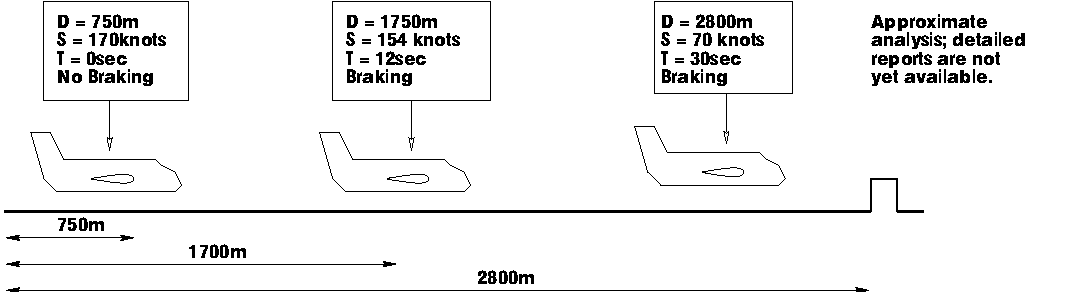
\includegraphics[scale=0.9]{\rootdir/safety/figures/okecie}
   \caption{The Lufthansa A320-200 at Okecie airport, Warsaw.}
   \label{fig:safety:okecie}
  \end{figure}




  \subsubsection*{Braking logic: Landing an A320 normally}

 Figure~\ref{fig:safety:AirbusSystems} presents an architectural view of the A320 braking system. The weight on the wheels (WoW) and the altitude (measure by the altimeter) are the two inputs.

  \begin{figure}[!h]
    \centering
    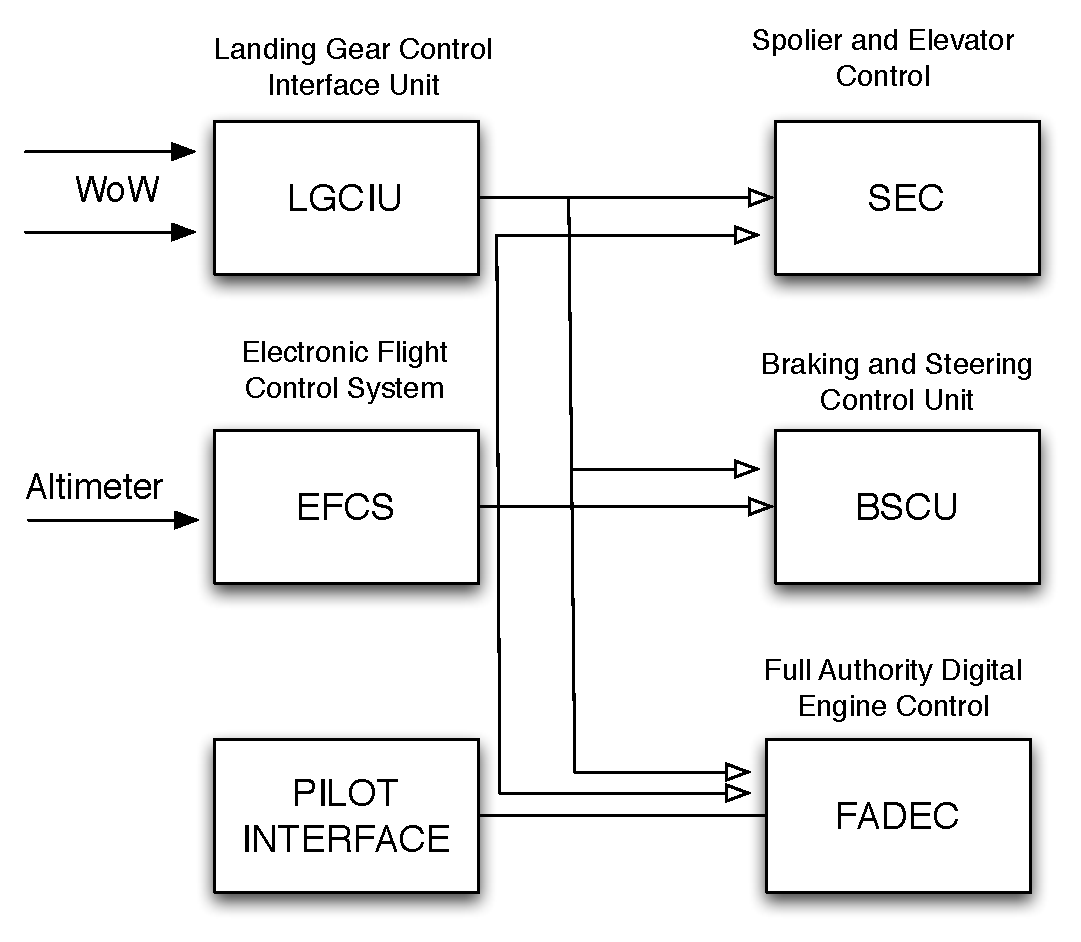
\includegraphics[width=0.75\textwidth]{\rootdir/safety/figures/AirbusSystems}
    \caption{Braking system for an A320 landing normally}
    \label{fig:safety:AirbusSystems}
  \end{figure}

The logic of the braking system is as follows:


   \hspace{2em}   brake if and only if:

   \hspace{6em}    (WoW $>$ 12 tonnes) \emph{and}

   \hspace{6em}   (wheels spinning $>$ 72 km/hr \emph{or}

\vspace{-2mm}

   \hspace{8em} (wheels spinning \emph{and} radia alt $<$ 10 feet ))




%------------------------------------------------------------
%%
%%    Okecie Accident Sequence
%%



  \subsubsection*{The Okecie accident sequence}



\begin{enumerate}

\item The crew were informed that the wind on the ground was coming
  from the right and slight in front of the aircraft at 10 knots.  The
  crew were not informed that during the final approach the wind
  changed to a tail wind of 25 knots.

\item To compensate for the cross wind coming from the front of the
  aircraft the crew had chosen a landing speed of 152 knots rather
  than the standard 132 knots which was normal procedure in bad
  weather of this kind.


\item Expecting a side wind the crew had banked the plane to the
  right.  The result was that only the right landing gear touched the
  runway.  The left gear did not come down for a further 9s.

  A/G is indicated by both WOW switches.  The LGCIU could not signal
  A/G and so the SEC did not deploy the ground spoilers and the FADECs
  did not deploy reverse thrust.

\item The wheel that had made contact with the runway was aqua-planing
  and so did not rotate at the required speed corresponding to 72
  knots.  Thus the other condition for the SEC to deploy spoilers was
  not true.

  \end{enumerate}


%------------------------------------------------------------
%%
%%    Okecie Accident Sequence
%%



  \subsubsection*{Conclusions from the Okecie accident}

  There is a lack of published evidence in the case of the Kulmbach
  accident at Okecie.  Some conclusions are drawn by Mellor \cite{mellor1994cad}:

 \begin{itemize}

  \item The crash was not due solely to pilot error.  The pilot may have
  contributed to the accident by selection of the landing speed but the
  Kulmbach should have been able to stop in the distance even at the
  speed of 170 knots. 

  \item The drainage of water from the runway and the weather conditions
  were necessary conditions for the accident but probably not sufficient
  on their own.  Several other aircraft landed successfully on runway 11
  both before and after the Kulmbach in the similar conditions. 

  \item The A320 systems may have performed to specifications but did
  not behave as required.  In retrospect, the braking logic is
  restrictive. 

  \end{itemize}

\emph{Again, it was the failure of the entire system that led to the accident}.


%------------------------------------------------------------


  \subsection{The role of accident analysis in safety engineering}


Accidents, and the study of accidents, are an important part of safety engineering. The most useful way to identify hazards in safety-critical systems is to look at similar systems and study the factors that contributed to accidents (and incidents) in those systems, and to specify safety requirements from both these and the system models (see Figure~\ref{fig:safety:RolesAccidents}).  Accident analyses are used during Preliminary Hazard Analysis (for example during HAZOP) to understand potential accidents, causes  consequences and risks.



  \begin{figure}[!h]
    \centering
    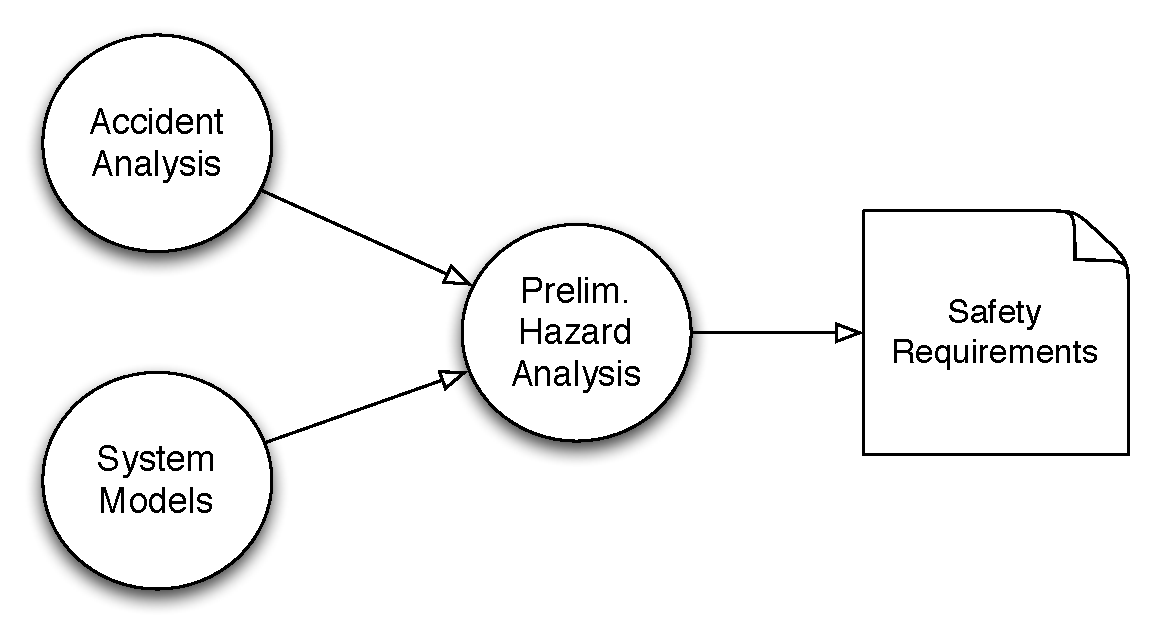
\includegraphics[scale=0.6]{\rootdir/safety/figures/RolesAccidents}
    \caption{The role of accidents in safety engineering}
    \label{fig:safety:RolesAccidents}
  \end{figure}  



  \subsubsection*{Analysing Accidents: Event Chains}

  The common method for analysing accidents is to create an \emph{event
    chain} leading back to a set of accident causes. Figure~\ref{fig:safety:EventChain} shows an example of an event chain for an accident in a steam boiler.

  \begin{figure}[!h]
    \centering 
    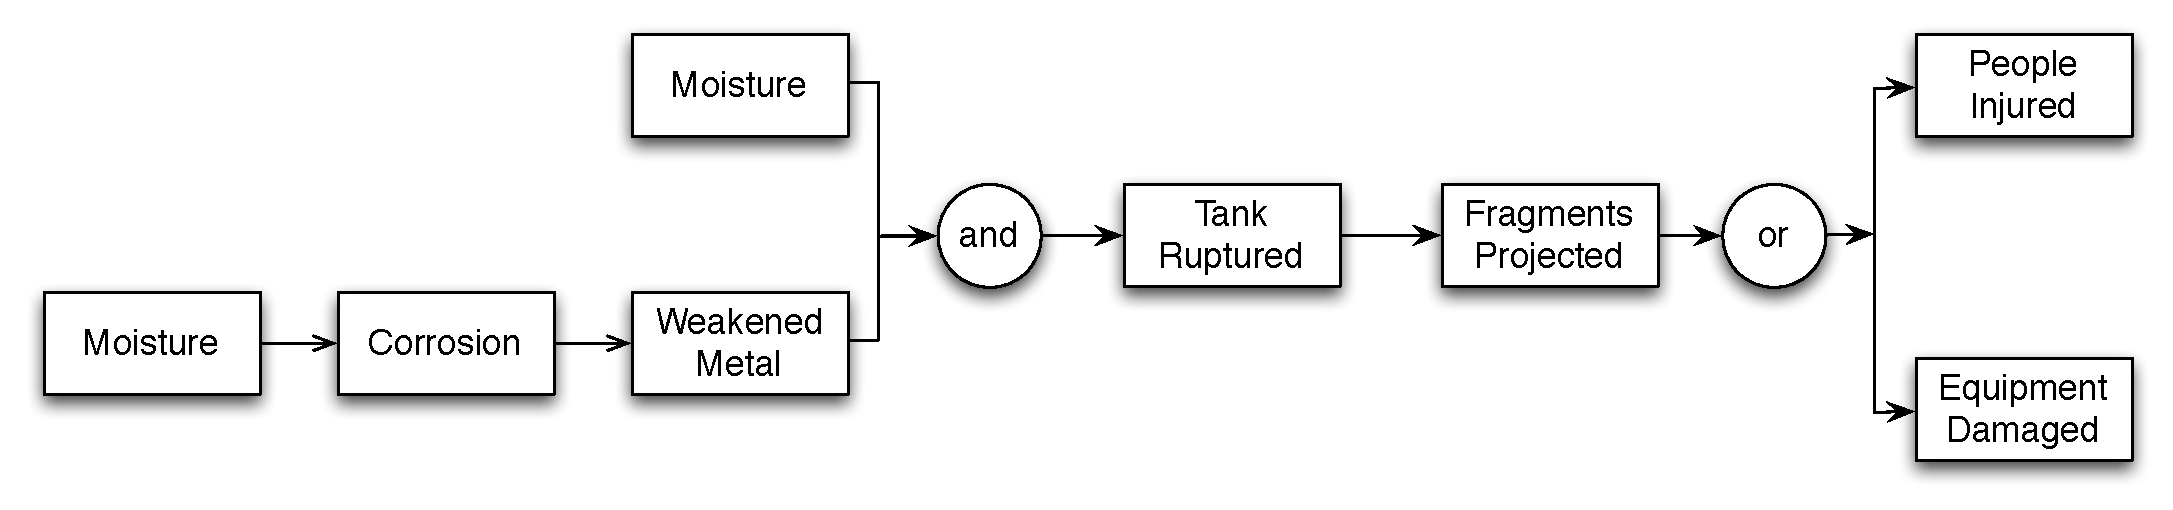
\includegraphics[scale=0.45]{\rootdir/safety/figures/EventChain}
    \caption{An event chain for a steam boiler}
    \label{fig:safety:EventChain}
  \end{figure}

  Each event in the chain is the cause of the next; for example, moisture is
  the cause of corrosion, corrosion is the cause of weakened metal in the
  boiler, moisture \emph{and} weakened metal is the cause of a ruptured tank, etc.

  \subsubsection*{Causality}
  


  {\em When can it be said that event A causes event B}?



  In accident analysis one common way is through the \emph{counterfactual} definition of causality.


 \begin{definition}
  A {\em counterfactual} is commonly defined as a conditional expressing what could have happened under different conditions, but did not happen. It is typically expressed in the
  subjunctive mood: a conditional (or {\em if-then})
  statement indicating what would be the case if its antecedent were
  true although it is not true.
  \end{definition}

  As an example, consider the counterfactual: ``They would have done better on their assignments, if they had first done the workshops'' (take a hint from this).


In accident analysis, ``{\em A causes B}'' if we assume that {\em A}
did not occur then {\em B} would not have occurred. Note that this does not mean that \emph{A} is the sole cause of \emph{B}. As in the accidents described above, often multiple factors contribute in unlikely sequences to cause a single accident.




  \subsubsection*{Counterfactuals and Causality}


  In the steam boiler example we would reason as follows:
  \begin{quote}
    \emph{If the metal had not been corroded then the metal would not have
    been weakened.}
\end{quote}

The metal was corroded but the counterfactual deals with what {\em
  could} have been --- in this case, if we remove the corrosion then
we can imagine that the metal would not have been weakened (based on
our knowledge of corrosion and metal).
Consequently the counterfactual is true and we conclude that the
corrosion of metal {\em causes} the weakening.

  The essential nature of counterfactuals in accident analysis is the
  imaged absence of one of the precondition events leading directly to
  the event being studied.
  If the consequent is true when we imagine that the antecedent is
  true then the counterfactual is true --- that is, we imagine the
  absence of the cause {\em A} and if the event {\em B} no longer
  occurs then {\em A causes B}.


  \subsubsection*{Counterfactuals and correlation}
  
  We must also be careful not to confuse causal relationship with {\em
    correlations}.

  \begin{quote}
    \emph{If the were the case that the barometer falls then a storm would occur.}
  \end{quote}

  In this case the barometer falling and the storm occurring are not
  causally linked --- the counterfactual is incidental and \emph{not
    true}.





  \section{Tools and techniques for safety engineering}

 The aim of this section is to examine some of the concepts, tools
  and techniques involved in safety engineering in a bit more depth. 


The problem in safety engineering is to develop -- with a high level of assurance:

\begin{itemize}

  \item Systems that do not lead to unintended harm or loss;

  \item Systems that continue to function in the presence of component
  faults;

  \item Systems that perform within hard real-time bounds; and 

  \item Systems that protect data.

\end{itemize}


\subsection{Safety standards and safety lifecycles}


  Software engineering for safety critical systems involves numerous
  standards each of which requires additional activities in order to
  guarantee due care with safety critical functions.

  For example, in IEC--61508, the safety lifecycle is used to
  identify:
  \begin{itemize}

  \item key activities where safety analysis techniques are used; and
    
  \item the relation between safety critical analysis methods and
    traditional lifecycle processes.
    
  \end{itemize}


 Engineering for safety, like engineering for other product attributes such as performance, correctness, and usability, is something that must be done over the entire lifecycle. Figure~\ref{fig:safety:ToolsAndTechniques} shows a possible safety engineering process, and notes some of the techniques and types of methods used in safety engineering.

  \begin{figure}[!h]
   \centering
    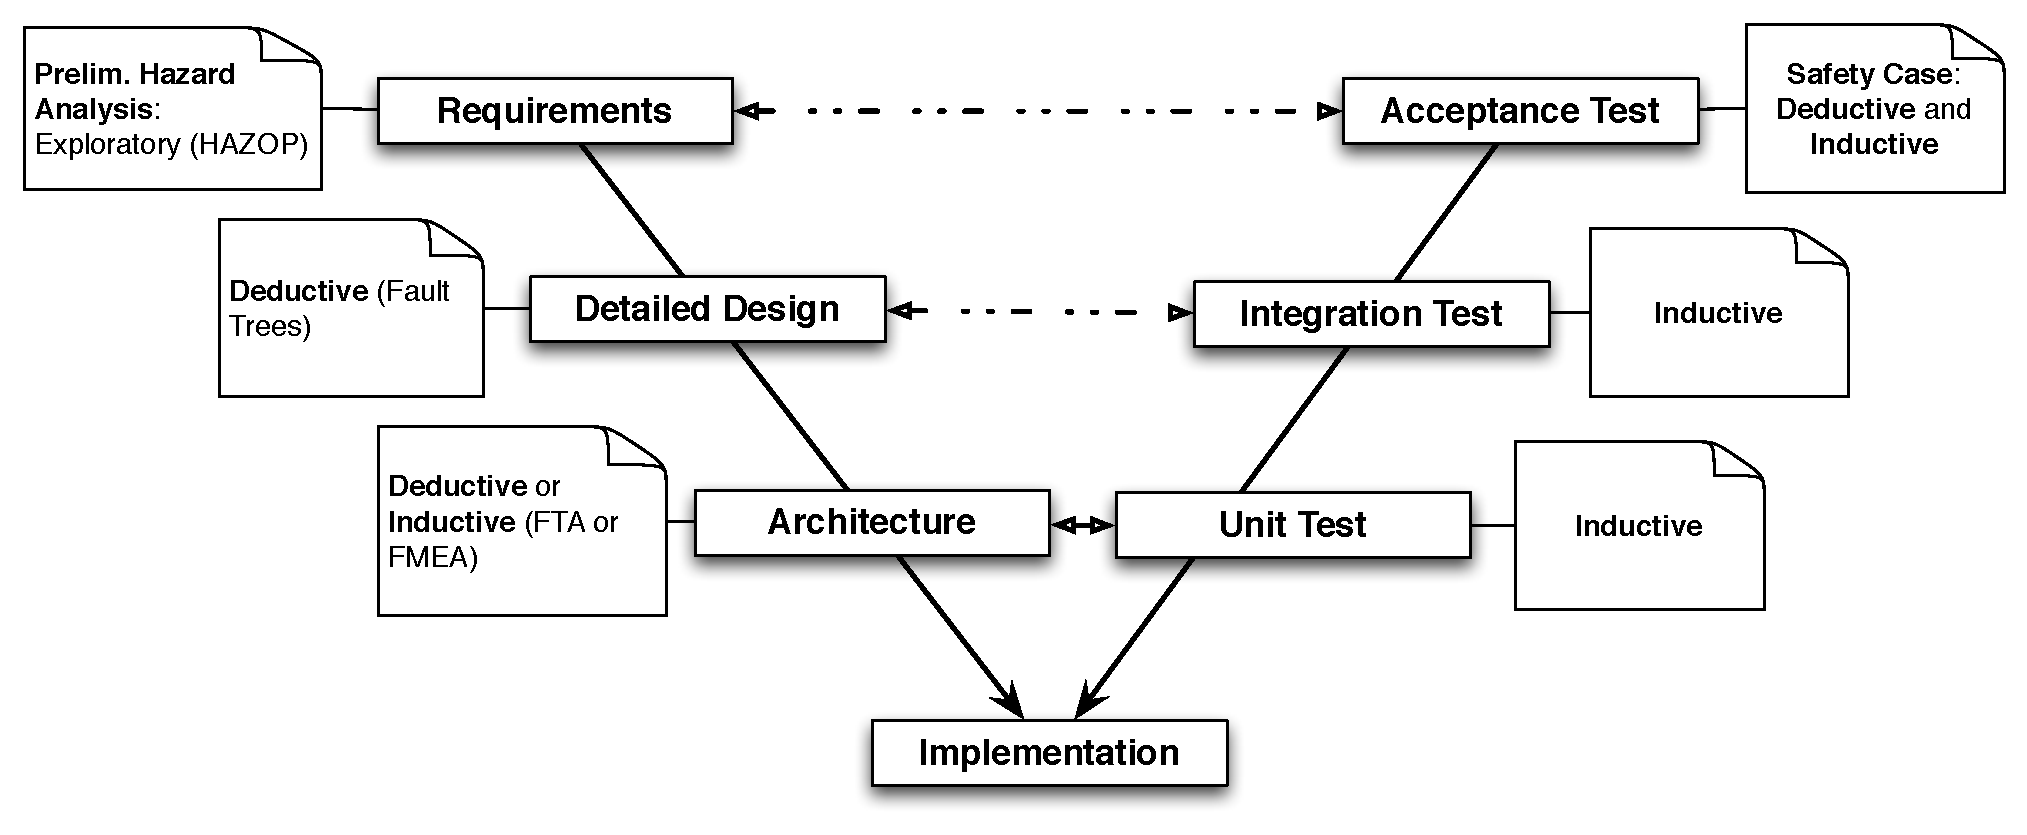
\includegraphics[scale=0.45]{\rootdir/safety/figures/ToolsAndTechniques}
    \caption{A safety engineering process}
   \label{fig:safety:ToolsAndTechniques} 
  \end{figure}
  
 For each project, or each iteration of a project, the phases of requirements, design, and implementation will have corresponding verification and validation techniques. At the requirements phase, the focus is more on exploratory hazard analysis to determine what could go wrong, while at later phases, it is about designing the system to prevent these.

  In the remainder of this chapter, we look at some safety engineering techniques. First, we present a more general overview of preliminary hazard analysis.



  \subsection{Preliminary hazard analysis}

 A \emph{preliminary hazard analysis} is used to identify the hazards and accident scenarios associated with a new system. It is essentially an information collation and filtering exercise, and is usually the
first activity carried out in the safety lifecycle. Preliminary hazard analysis methods ask: ``What
possible accidents or incidents could occur?''

In this section, we look at some of the basic concepts in preliminary hazard analysis.


  \subsubsection*{Phase 1 --- Preliminary hazard identification}

   This is the phase that identifies the hazards and accident scenarios 
    	associated with the new system. 


  \begin{itemize}
    \item \textbf{Inputs -- Information sources}
     
        \begin{itemize}

            \item \emph{Incident and hazard data:} previous in-service 
            incident and accident data of similar systems (usually as 
            checklists).
             
            \item \emph{Analyses:} previous dependability analyses for 
            similar systems.
             
        \end{itemize}
         
    \item \textbf{Method}
    
        \begin{itemize}
        
            \item \emph{Group based:} members experienced in the domain. This is important because people who have domain knowledge and knowledge about accidents are far more likely to think of accidents for the new system.
            
            \item \emph{What ifs:} hypothesise safety related 
            difficulties.
        
        \end{itemize}
        
    \item \textbf{Output}
    
        \begin{itemize}

            \item \emph{Preliminary hazard list:} a list of all hazards, their causes.
        
        \end{itemize}

\end{itemize}

\subsubsection*{Phase 2 --- Preliminary Hazard Analysis (PHA)}

 This occurs after the preliminary hazard identification and usually 
    at the later stages of requirements analysis and early stages of 
    design. It has the following properties:

\begin{itemize}

    \item Possibly included into preliminary design reviews.
    
    \item Early identification of hazards and causes in designs.
    
    \item It is a poorly defined method:
    
        \begin{itemize}
	\setlength{\itemsep}{2pt}\setlength{\topsep}{2pt}
        
            \item uses brainstorming and questionnaires; and
            
            \item depends on experience and domain knowledge.
        
        \end{itemize}

    \item Checklists are commonly used, in an attempt to make the method more systematic, and less reliant on experience and domain knowledge.

\end{itemize}


\begin{description}
   \item[Inputs]\mbox{}\\[-2ex]
    
        \begin{itemize}
	\setlength{\itemsep}{2pt}\setlength{\topsep}{2pt}
        
            \item design (or perhaps a detailed requirements model).
            
            \item preliminary hazard list
        
        \end{itemize}
    
    \item[Outputs]\mbox{}\\[-2ex]
    
        \begin{itemize}
       
            \item list of causes for hazards based on the design.
           
            \item risk assessment and risk classes (provisional).
            
            \item integrity levels (provisional).
            
            \item target failure rates (provisional).

        \end{itemize}

\end{description}

%-------------------------------------------------------------------------
%%
%%
%%    Hazard logs
%%


  \subsubsection*{Hazard Logs}

The results of the preliminary hazard identification and preliminary 
hazard analysis form the basis of a \emph{hazard log}.

\begin{definition}
A \emph{hazard log} lists the hazards, their causes and their 
    severity,  as well as other data such as target frequencies or hazard 
    types.
 It is a living document.  It evolves during the course of the
    safety analysis, and can be part of the common literature in special
    fields such as avionics.
\end{definition}

For example, a preliminary hazard analysis may be summarised in the 
following hazard log.

\begin{center}
   \begin{tabular}{lllllll}
     \toprule
     \textbf{Ref.} & \textbf{Hazard} & \textbf{Frequency} &
     \textbf{Severity} & \textbf{Cause} & 
     \textbf{Integrity} & \textbf{Target} \\
     & & & & & \textbf{Level} &  \\
     \midrule
     \ldots & & & & &  & \\
     \ldots & & & & &  & \\
     \bottomrule
    \end{tabular}
\end{center}


  \subsubsection{Risk}


 \emph{Risk} is function of the severity of a hazardous event and the
 likelihood of it occurring. The \emph{frequency} of the event is the
 probability that the event occurs in a given period of time.
        
  \subsubsection*{Assessing Risk}

 To arrive at a qualitative risk assessment, the idea is to
  assess consequences against frequencies.  Standards usually provide
  a table for this.

    The safety standard IEC -- 61508 classifies consequences into: 
      \begin{center}
            \begin{tabular}{ll} 
              catastrophic & critical \\
              marginal     & negligible
            \end{tabular}
        \end{center}

    It classifies frequencies into:
        \begin{center}
            \begin{tabular}{lll}
                frequent & probable & occasional \\
                remote   & improbable & incredible
            \end{tabular}
        \end{center}

%-------------------------------------------------------------------------
%%
%%
%%   Risk classes and their interpretation
%%


From these two classifications, the standard defines the following table, which classifies each consequence/frequency pair into one of four \emph{risk classes}.

\begin{center}
    \begin{tabular}{lcccc}
	\toprule
	Frequency & \multicolumn{4}{c}{Consequence}\\\cmidrule{2-5}
                  & Catastrophic & Critical & Marginal & Negligible \\
	\midrule
	Frequent & I & I & I & II \\
	Probable & I & I & II & III\\
	Occasional & I & II & III & III\\
	Remote & II & III & III & IV \\ 
	Incredible & IV & IV & IV & IV \\
	\bottomrule
    \end{tabular}
\end{center}

The four risks classes, according to IEC -- 61508, are:


\begin{tabular}{ll}

\textbf{Class I} & Intolerable risk.\\

\textbf{Class II} & Undesirable risk and tolerable only if risk
	  	reduction is impractical.\\

\textbf{Class III} & Tolerable risk if the cost of risk reduction
		would exceed the improvement gained.\\

\textbf{Class IV} & Negligible risk.

\end{tabular}

Using this, we can interpret that frequent events with a catastrophic must not be tolerated, while incredibly rare events in general can be tolerated.


%-------------------------------------------------------------------------
%%
%%
%%    Integrity Levels
%%


  \subsubsection{Integrity Levels}

  \begin{definition}
   \emph{Safety integrity} is the likelihood of a safety related 
    system satisfactorily performing the required safety functions under 
    all stated conditions.
   \end{definition}


     For example, a system with known failure rates for subsystems:

    \begin{center}
        \begin{tabular}{ll}
        \toprule
        \textbf{Integrity} & \textbf{Probability of failure to} \\
        \textbf{Level}    & \textbf{perform system function}   \\
        \midrule
        4 & $\ge 10^{-5}$ to $<10^{-4}$ \\
        3 & $\ge 10^{-4}$ to $<10^{-3}$ \\
        2 & $\ge 10^{-3}$ to $<10^{-2}$ \\
        1 & $\ge 10^{-2}$ to $<10^{-1}$ \\
        \bottomrule
        \end{tabular}
    \end{center}

    \textbf{Note:} the distinction between risk classes and 
    integrity levels.  Risk classes are assigned to hazards.  Integrity 
    levels are assigned to systems.
    


%-------------------------------------------------------------------------
%%
%%
%%    Assigning Integrity Levels
%%


  \subsubsection*{Assigning Integrity Levels}


   It is not always possible to remove hazards entirely. Safety engineers must instead reduce hazard risks to tolerable risk levels. The amount of risk reduction determines the integrity level.  
    The more that the system is required to reduce the risk of hazards 
    the higher the system's integrity level.
    
    There are a number of ways of assigning integrity levels to 
    subsystems, and these can be broken into two categories:

        \begin{enumerate}

            \item Quantitative methods -- first determine the
            uncontrolled risk and then target risk levels numerically,
            by analysing the failure rates of subsystems from similar
            situations;
            
            \item Qualitative methods -- use risk graphs to determine
            risk qualitatively.
        
        \end{enumerate}



  Some standards, such as IEC-61508, provide for integrity levels which
  are set according to the severity of the accident.
%-------------------------------------------------------------------------


  \section{Hazard Analysis Methods}

Hazard analysis methods fall into three categories: 

\begin{enumerate}

 \item \emph{exploratory}: these methods use expert knowledge and some systematic techniques to imagine potential hazards and their impacts;

 \item \emph{causal}: these methods work from system designs and try to deduce what failures are possible from this;  and
 
 \item \emph{consequence}: these methods work backwards from possible failures to see how they could occur.

\end{enumerate}

Table~\ref{tab:safety:hazard-analysis-methods} summarises these three types of methods. In the remainder of this chapter, we will explore the three methods listed as examples in Table~\ref{tab:safety:hazard-analysis-methods}.

\begin{table}[!h]
\centering
\begin{tabular}{lp{5cm}p{7cm}}
\toprule
{\bf Technique} & {\bf Example Methods} & {\bf Good For \ldots}\\
\midrule
Exploratory & HAZOP (Hazard and Operability Studies) & Exploring
possible hazards, their causes and for completeness, but is 
labour intensive and hard to change. \\[2mm]
Causal & Fault Trees & This is the classic deductive approach and is
good for determining what combinations of component failures lead to
hazards.\\[2mm]
Consequence & FMEA (Failure Modes and Effects Analysis) & This is the
classical inductive approach used for working from component failures
(failure modes) back to hazards and is good for verifying ideas and
designs.\\
\bottomrule
\end{tabular}
\caption{Types of hazard analysis methods.}
\label{tab:safety:hazard-analysis-methods}
\end{table}


  \subsection{HAZOPS}
  
\emph{HAZard and OPerability Studies} (HAZOPS) is a technique that originated in the chemical processing industry. It has been adapted to many other industries and specifically in software engineering to software HAZOPS and --- surprisingly --- the study of interfaces in human-computer interaction.

A HAZOP study is a well-established technique for preliminary hazard
  analysis (PHA). The process of identifying hazards requires creativity, lateral thinking, and expert knowledge. The HAZOPS method was introduced into software engineering to provide some repeatable and systematic process into hazard analysis.

The basic technique is straightforward: a system consists of some behaviour. A HAZOP study explores the behaviour by taking a set of generic \emph{guidewords} that describe some alternative to intended behaviour, and exploring what hazards could occur if that alternate behaviour occurred.

{\bf Note:} this is different to testing where we wish to find deviations from {\em specified behaviour}.

\subsubsection*{Guidewords}

The guidewords for every HAZOP study are the same\footnote{Although there is nothing to prevent software engineers from adding or removing guidewords.}, and are listed in Table~\ref{tab:safety:hazop-guidewords}.

\begin{table}[!h]
\centering
\begin{tabular}{lp{11cm}}
 \toprule
      \textbf{Guide Word} & \textbf{Deviation}\\
 \midrule
      NO or NONE & This is the complete negation of the design intention. No
      part of the intention is achieved and nothing else happens.\\
      MORE & This is a quantitative increase.\\
      LESS & This is a quantitative decrease.\\
      AS WELL AS & All the design intention is achieved together with additions.\\
      PART OF & Only some of the design intention is achieved. \\
      REVERSE & The logical opposite of the intention is achieved.\\
      OTHER THAN & Complete substitution, where no part of the original
      intention is achieved but something quite different happens. \\
    EARLY  & Something happens earlier than expected relative to clock time.\\
    LATE & Something happens later than expected relative to clock time. \\
    BEFORE & Something happens before it is expected, relating to
    order or sequence.\\
    AFTER & Something happens after it is expected, relating to order or sequence.\\
\bottomrule
\end{tabular}
\caption{HAZOPS guidewords}
\label{tab:safety:hazop-guidewords}
\end{table}


\subsubsection*{Roles}

There are several roles that can take part in a HAZOP study, including:

  \begin{enumerate}

    \item A Team leader who is responsible for:
      \begin{itemize}
      \item Planning and Preparation.

      \item Chairing the HAZOPS meetings.

      \item Signing any documentation.

      \item Ensuring follow-up work is completed.

      \end{itemize}
    \item Recorder who is responsible for:
      \begin{itemize}
      \item Documenting the analysis.

      \item Participating in the study.

      \end{itemize}

\item Designers 
    \begin{itemize}

   \item Understand and explain the (potential) design.
 
    \item  Answer questions about the process.

    \end{itemize}

\item User(s) 

\begin{itemize}
    \item May be operators, or representatives of other user
    groups such as maintainers of the system.

    \item Supply information about the context in which the system
    will be used.

    \item  Help decide issues that may affect safety.
\end{itemize}

 \item Expert(s). The key function of experts is to {\em explore}:

  \begin{itemize}

   \item Ask questions.

   \item Suggest deviations, causes and effects.

  \end{itemize}

\end{enumerate}
  
\subsubsection*{Process}

\begin{figure}[!h]
\centering
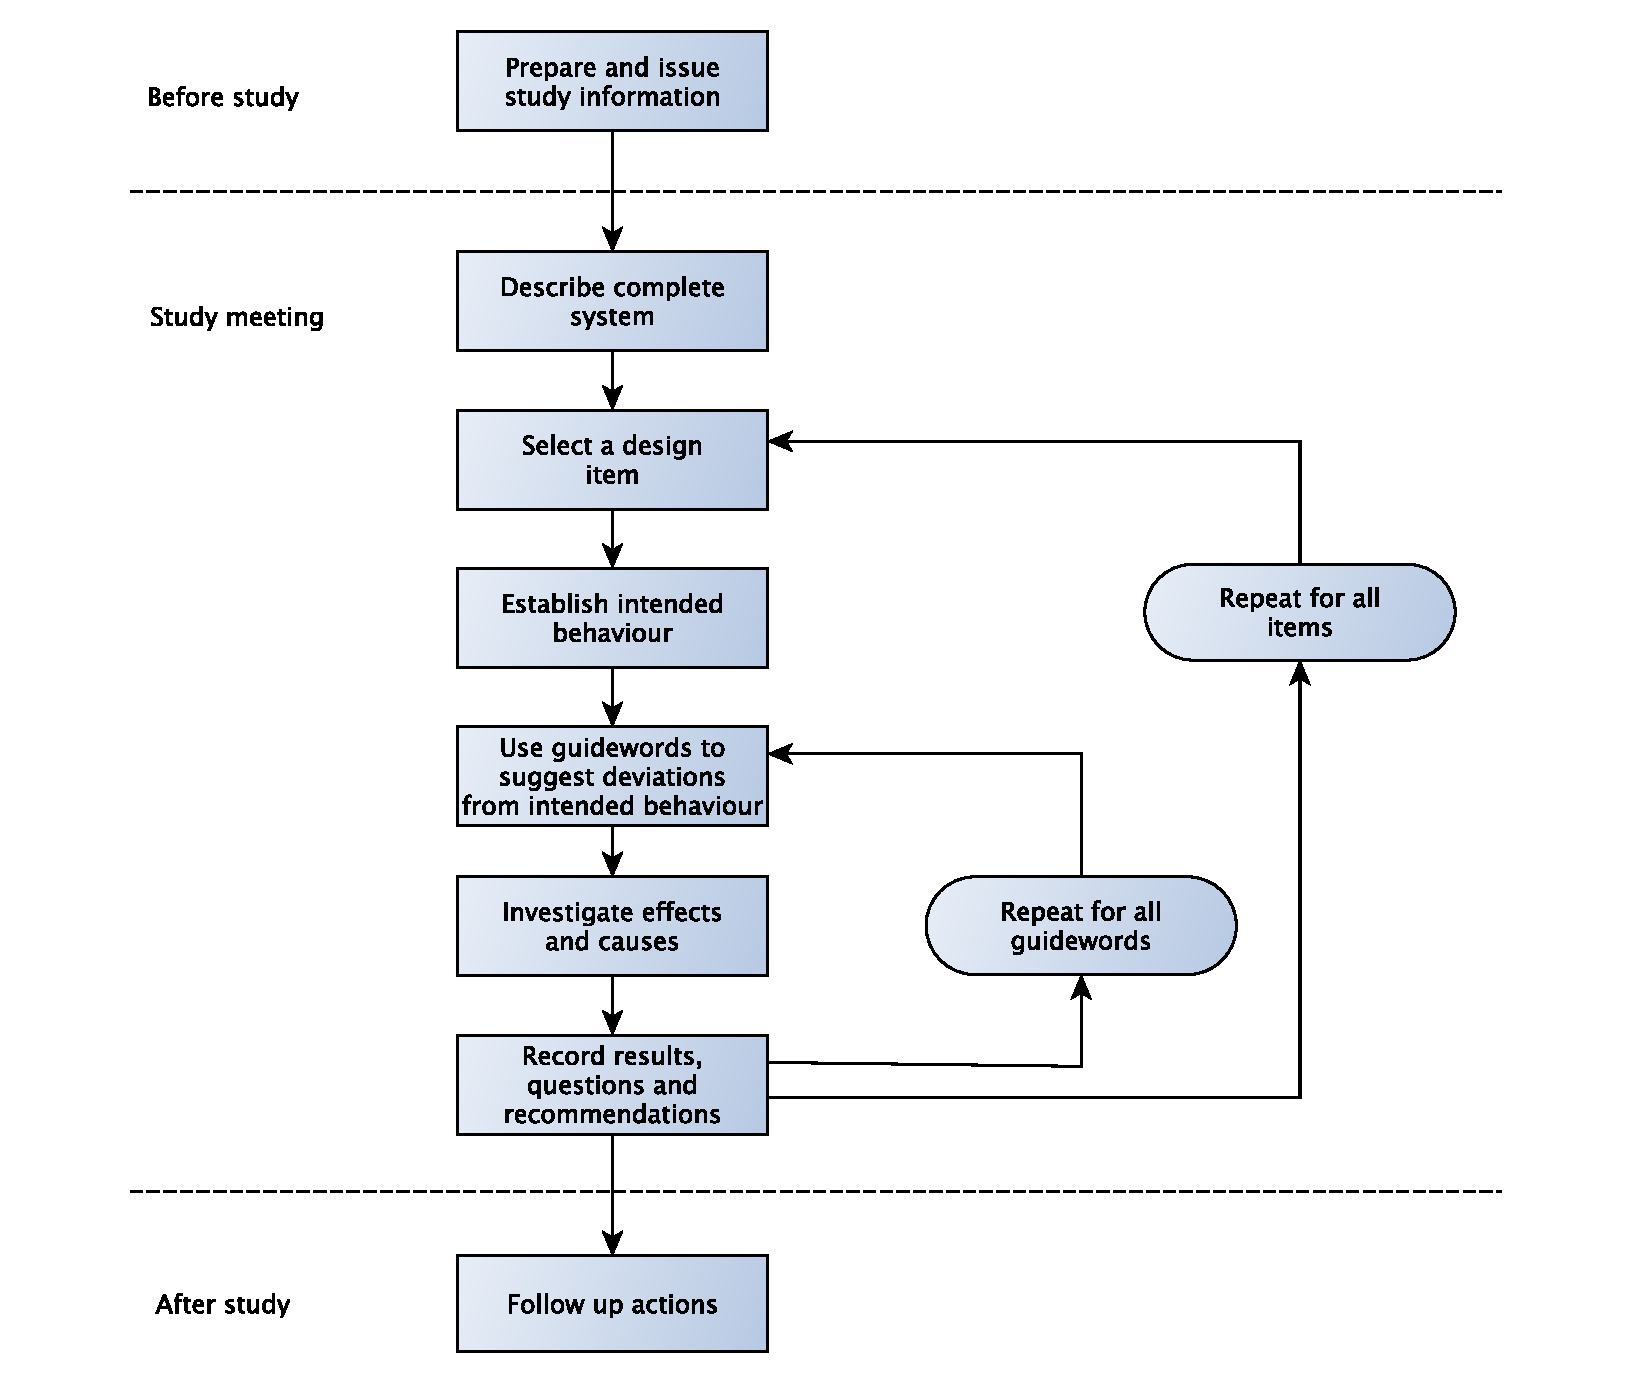
\includegraphics[scale=0.55]{\rootdir/safety/figures/HAZOP-process}
\caption{A HAZOP study process.}
\label{fig:safety:HAZOP-process}
\end{figure}


The process for a HAZOP study is outlined in Figure~\ref{fig:safety:HAZOP-process}, taken from \cite{mcdermid1995experience}. From this figure, we can see that each design item, such as an event in a process, or a transition in a state machine, is inspected. For each item, the item is analysed using the HAZOP guidewords. 

For example, consider our earlier idea of brake-by-wire system for a car. One design item contains the intended behaviour that, when the brake pedal is pushed, a signal must be sent to the ECU immediately to let it know that this event has occurred. Using a HAZOP study to analyse what happens if the systems deviates from intention, we can apply the guidewords NONE, EARLY, and LATE, and then reason the following:

\begin{itemize}
 
 \item NONE: If no signal is sent, the ECU will not know that the brake has been pushed, so will not send the signal to apply the brakes to the wheels. This will result in the vehicle not decelerating, ultimately resulting in a hazard.

 \item EARLY: We want the signal to be sent immediately, so a signal cannot be sent early, and therefore, no hazard occurs.

 \item LATE: If the signal is sent late, the ECU will process it late and send a signal late to the brakes. This will result in the vehicle decelerating later than anticipated, ultimately resulting in a hazard.

\end{itemize}


The result is a log of the entire analysis. For each design item + guideword pair that may result in a hazard, the following details are recorded:

\begin{enumerate}

 \item The deviation from intent (the interpretation of the design item + guideword for this system).

 \item The causes of the deviation.

 \item The consequences of the deviations.

 \item Any safeguards that are in place to prevent the deviation or its cause.

 \item A list of recommendations for mitigating the problem.

\end{enumerate}


A template/examples for this is shown in Table~\ref{fig:safety:HAZOP-log}.

\begin{table}[!h]
\centering
\begin{tabular}{lllllll}
\toprule
\textbf{ID} & \textbf{Guideword} & \textbf{Deviation} & 
 \textbf{Causes} & \textbf{Consequences} & \textbf{Safeguards} &
 \textbf{Recommendations}\\
\midrule
 1.1 & NONE & \ldots & \ldots & \ldots & \ldots & \ldots\\
 1.2 & EARLY & \ldots & \ldots & \ldots & \ldots & \ldots\\
 1.3 & LATE & \ldots & \ldots & \ldots & \ldots & \ldots\\
 \ldots & \\
\bottomrule
\end{tabular}
\caption{A template for a HAZOP log.}
\label{fig:safety:HAZOP-log}
\end{table}

\subsubsection*{Limitations}

There are several limitations with using HAZOPS as preliminary a hazard analysis technique:

\begin{enumerate}

 \item It requires a well-defined description of the intended behaviour. In some projects, this may not be available until quite late.

 \item It is extremely time and resource intensive. Several people in a team analysing every design item for every guideword is time consuming, and the people in the team are generally highly experienced.

 Despite this, the process is creative and challenging, and many people find it rewarding and interesting. 
 Not me though \ldots

 \item To conform to most safety standards, to devise a safety case, and to enable traceability of decisions, the result of the entire analysis must be recorded. That is, the outcomes of each guideword + design item pair must be recorded, including causes, consequences, and recommendations for mitigating the problem.
  This results in large amounts of documentation that need to be  reviewed and maintained.

 \item It focuses on single failures that cause of deviation from intent. However, an accident can occur due to a series of unlikely circumstances along a chain of events in a system. 
 Despite this, the use of guidewords may prompt system designers to consider chains of deviations.

\end{enumerate}

\begin{example}
The following example of a \emph{stepper motor} HAZOP study is taken from Wei and Zhangjin \cite{wei-hazop-report}.

A stepper motor is a electric motor used for rotation of mechanical parts. The rotation is divided into discrete number of equal size steps. The position of the motor can therefore be determined without the use of sensors for feedback, provided the motor size is known. Figure~\ref{fig:safety:StepperMotor} shows the workings of a stepper motor: a single step moves the teeth around until they are locked in, so counting the steps means that the position of the motor is known. The system is real-time, so when the controller of the motor sends a message for it to rotate, power on, etc., it must do it within a specified (and short!) time frame.

\begin{figure}[!h]
\centering
  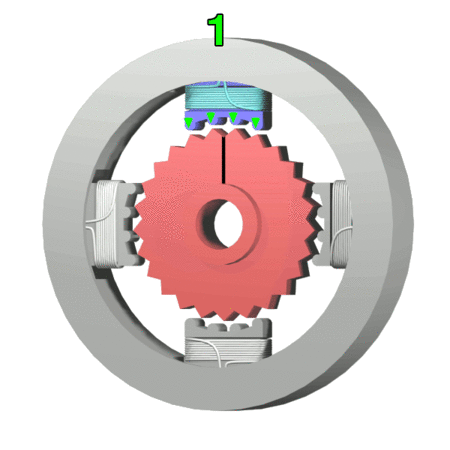
\includegraphics[scale=0.24]{\rootdir/safety/figures/StepperMotor-0}
  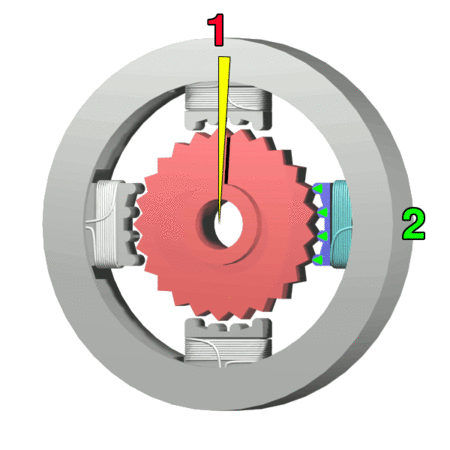
\includegraphics[scale=0.24]{\rootdir/safety/figures/StepperMotor-1}
  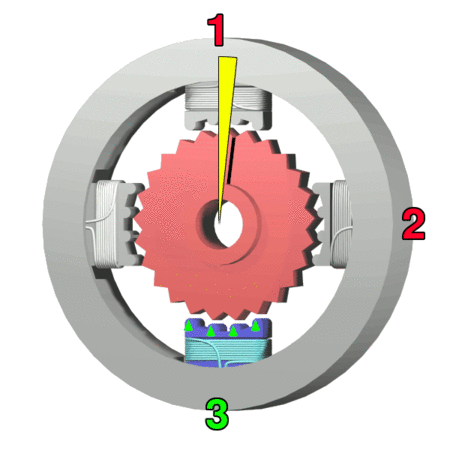
\includegraphics[scale=0.24]{\rootdir/safety/figures/StepperMotor-2}
  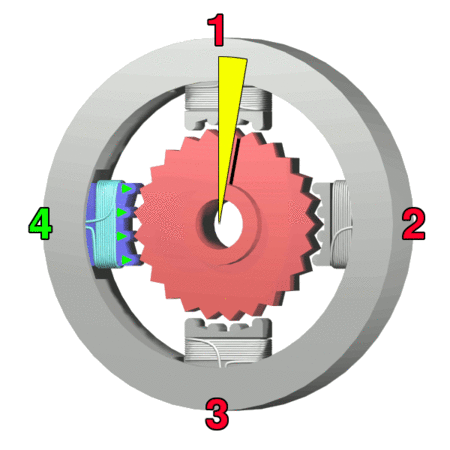
\includegraphics[scale=0.24]{\rootdir/safety/figures/StepperMotor-3}
 \caption{An overview of a stepper motor.}
 \label{fig:safety:StepperMotor}
\end{figure}

The controller uses a C interface to the control the library, shown in Figure~\ref{fig:safety:stepper-motor-interface}. Motor identifiers can be created, and a specified motor can be powered on/off, moved forward a number of steps, and braked.

\begin{figure}[!h]
\begin{verbatim}
    void write_lpt(struct motor_t *motor);
    struct motor_t stepper_motor_setup(int motor);
    void stepper_motor_power_on(struct motor_t *motor);
    void stepper_motor_power_off(struct motor_t *motor);
    void stepper_motor_move_steps(struct motor_t *motor);
    void stepper_motor_set_safe(struct motor t *motor);
    void stepper_motor_brake(struct motor t *motor);
\end{verbatim}
\caption{C interface for a stepper motor.}
\label{fig:safety:stepper-motor-interface}
\end{figure}

First, we need to infer what the deviations from intent are for each guideword:

\begin{center}
\begin{tabular}{llllllllll}
\toprule
 \textbf{Item} & \multicolumn{9}{c}{\textbf{Guidewords}}\\
\cmidrule{2-10}
     & NONE & MORE & LESS & EARLY & LATE & BEFORE & AFTER & REVERSE & ...\\
\midrule
Power  & No & Over  & Under  & Voltage  & Voltage  & --- & --- & Backflow\\[-1mm]
       & voltage & voltage & voltage & change & change &  & & \\[1mm]
 Step  & No & Less & More & --- & Late & --- & Wrong & Wrong \\[-1mm]
       & steps & steps & steps & & time &  & order & direction\\[1mm]
 Brake & No & Too & Too & Too & Too & Wrong & Wrong & Accel-\\[-1mm]
       & brake & quickly & slowly & early & late & order & order & erate\\
 \ldots & \multicolumn{9}{c}{\ldots}\\
\bottomrule
\end{tabular}
\end{center}

Now that we have the deviations from intent, we need to analyse what the possible hazards that arise as a consequence of these. We do just part of the functionality for moving the stepper motor:

\begin{center}
\begin{tabular}{llp{2cm}p{2cm}p{2cm}p{2cm}p{3cm}}\\
\toprule
\multicolumn{7}{c}{3.0 \texttt{stepper\_motor\_move\_steps(struct motor\_t *motor);}}\\
\midrule
\textbf{ID} & \textbf{Guideword} & \textbf{Deviation} & 
 \textbf{Causes} & \textbf{Consequences} & \textbf{Safeguards} &
 \textbf{Recommendations}\\
\midrule
 3.1 & NONE & No steps & No power to motor & Motor does not move &  & \\[2mm]
 3.2 & MORE & More steps & Power too high &  1. Motor goes too fast. 2. Motor may burn out. &  & Install a voltometer. Do not apply voltage is over a specified threshold\\[2mm]
 3.2 & LESS & Less steps  & Low power due to old wire or large resistor & Motor rotates too slowly &  & Install a voltometer. Raise an error is voltage is under a specified threshold\\
 \multicolumn{7}{c}{\ldots}\\
\bottomrule
\end{tabular}
\end{center}

From just these few guidewords, we have noted some potential hazards and provided recommendations for them. Clearly, from the report, some knowledge of stepper motors and their operation is required, even for this small part of the analysis.
\end{example}



\subsection{Fault Tree Analysis}

Fault trees are one of the classic deductive techniques for hazard analysis and also one of the most common deductive technique in  use today. Fault trees are typically drawn by working back from hazards to basic causes.  Fault trees are a graphical notation and consist of events and gates.

\subsubsection*{Event and gate symbols}

Figures~\ref{fig:safety:fault-tree-symbols} and \ref{fig:safety-fault-tree-gates} show the symbols that are used in fault-tree analysis, dividing into \emph{event} symbols and \emph{gate} symbols respectively.

\begin{figure}[!h]
  \centering
  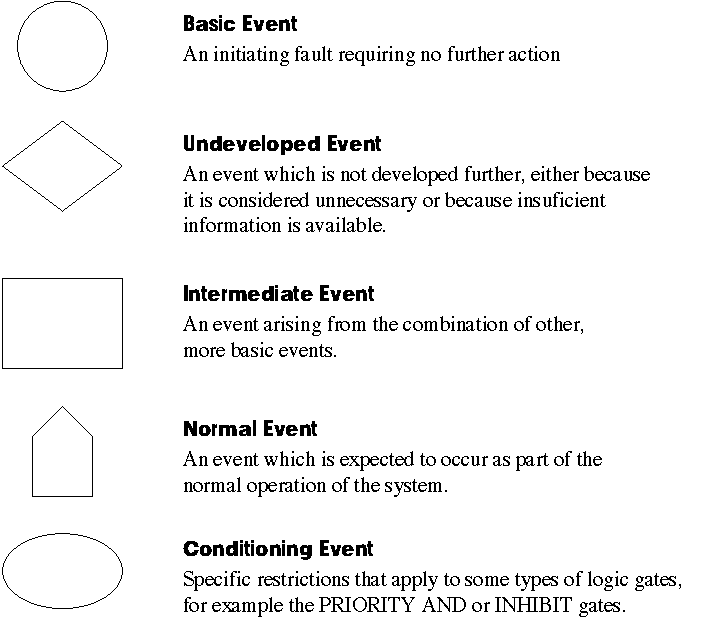
\includegraphics[scale=0.8]{\rootdir/safety/figures/fault-tree-symbols}
  \caption{Fault tree symbols}
  \label{fig:safety:fault-tree-symbols}
\end{figure}

\begin{figure}[!h]
  \centering
  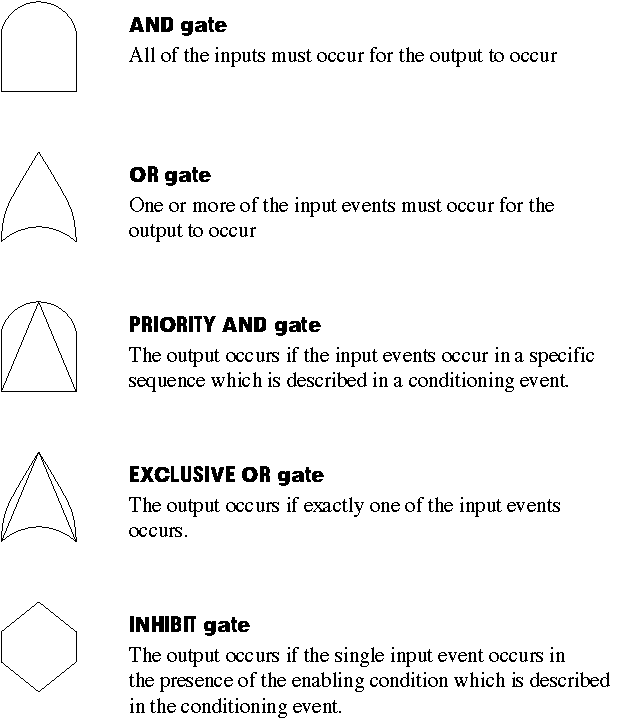
\includegraphics[scale=0.8]{\rootdir/safety/figures/fault-tree-gates}
  \caption{Fault tree gates}
  \label{fig:safety-fault-tree-gates}
\end{figure}

\subsubsection*{Method}

The basic method for working with fault trees is the following:

\begin{enumerate}

\item \emph{Select an event}: Initially we select top-level events,  which are typically the hazards, or events that  can lead to the hazards, identified in the PHA.

\item \emph{Identify immediate, necessary and sufficient causes of this
    event}:

  \begin{itemize}

  \item \emph{Immediate}: means that we need to avoid missing out
    intermediate events and should apply the ``\emph{think small}''
    principle;

  \item \emph{Necessary}: means determining those events which must
    occur for the top-level event to occur and these should be linked
    with an AND gate;

  \item \emph{Sufficient}: means getting those events which alone are
    sufficient to cause the top-level events on their own and these are linked with
    an OR gate.

   \end{itemize}

\item \emph{Classify intermediate events}:

      \begin{itemize}

      \item \emph{Basic event} requires no further decomposition.

      \item \emph{Compound defect}, which may one of (1) a primary failure, which is a simple component failure and may be classified as a basic event; (2) a secondary failure in which components fail because of external influences and this usually requires further investigation; or (3) command failure in which components receive incorrect signals and this always requires further investigation.

     \item \emph{System defect}, which is not attributable to a single component and always requires further investigation.

\end{itemize}

 \item \emph{Repeat as required.}
\end{enumerate}


\subsubsection*{Some heuristics}

There are some some heuristics that have evolved over time for the correct construction of fault trees:

\begin{enumerate}

\item All inputs to a gate should be defined before any one is examined
in more detail.

\item The output of a gate must never be directly linked to the input of
another gate -- all outputs of gates must go to events.

\item The text in event boxes should be complete in the sense that they
should always say what the event is and when it occurs.

\item Causes always chronologically precede consequences.

\end{enumerate}


\subsubsection*{Example: Chemical mixing plan}

Consider the simple chemical mixing plant shown in Figure~\ref{fig:FT-valve} and its accompanying fault tree \cite{mcdermid1995experience}.  The top-level event that leads to a hazard in this case is that the tank may overflow and cause environmental damage.

\begin{figure}[!h]
  \centering
  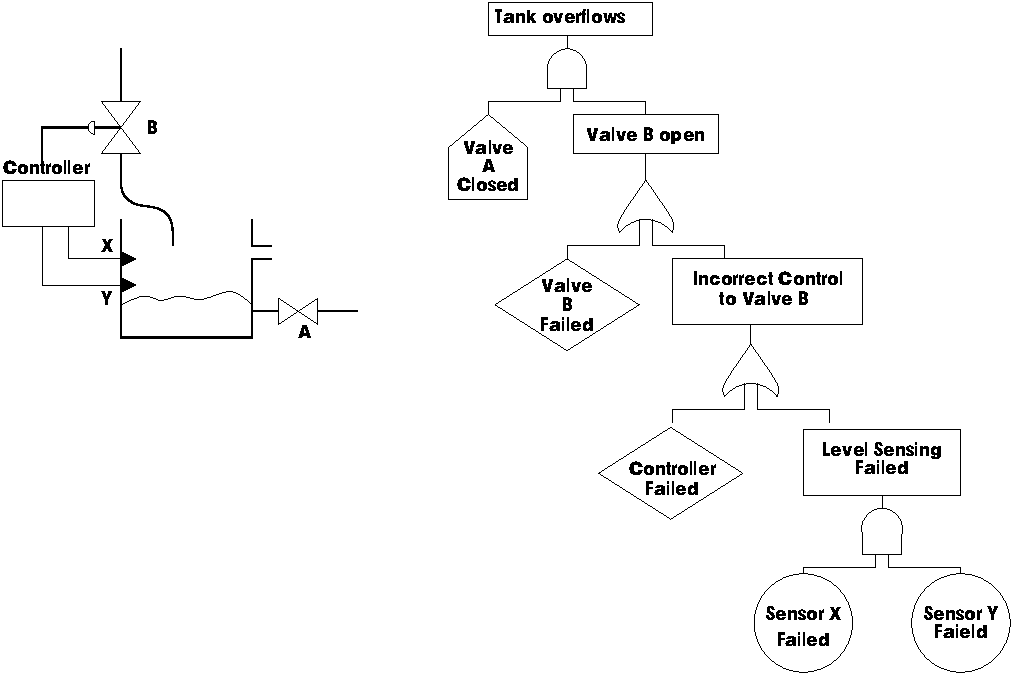
\includegraphics[scale=0.85]{\rootdir/safety/figures/fault-tree-valve}
  \caption{A design of a simple chemical mixing plant and its corresponding fault tree.}
  \label{fig:FT-valve}
\end{figure}


The immediate, necessary and sufficient causes of this event are that the valve marked A is closed and that the valve marked B is open. Note that these events must occur \emph{before} the tank overflows. The fault tree does not investigate the causes of the event ``\emph{valve A closed}'' further.

On the other hand, valve B is open if valve B has failed, which is a component failure but is not investigated further, or an incorrect signal has been sent to valve B, which is a command failure and must be investigated further.


\subsection{FMEA}
  
\emph{Failure Modes and Effects Analysis (FMEA)} is a tabular technique and is one of the most widely applied inductive (consequence analysis) techniques in industry.

The method specifies that safety engineers should focus on a single component failure, or failure mode, and work forward through subsystems to determine the consequence of the failure mode on the rest of the system.
There is a great deal of variation in FMEA practice and, like most hazard analysis methods, it is hard to give a general algorithm for conducting an FMEA.

\subsubsection*{Applications}

FMEA is good at identifying individual elements or operations within a system that render it vulnerable; that is, finding  single points of failure. Industries/organisations that frequently use FMEA include: consumer products, automotive, home appliances, aerospace, NASA, Department of Defence, and process industries (e.g.\ chemical processing).

\subsubsection*{Failure modes}

An FMEA is about identifying the \emph{failure modes} of a system.

\begin{definition}
A \emph{failure mode} is a manner in which a failure can occur, in terms of failure of the item function (such as a function to a sub-system or component) being studies.
\end{definition}

Typical failure modes are: 

  \begin{enumerate}
  \item Premature operation.
  \item Failure to operate at the required time.
  \item Failure to stop operation at the required time.
  \item Failure during operation --- and this is specific to the equipment.
  \item Degraded operational capacity.
  \item Excessive operational capacity.
  \end{enumerate}

There is a symmetry here between failure modes and the guidewords for HAZOPS; e.g.\ excessive operational capacity and the guideword ``MORE''.

\subsubsection*{Method}

\textbf{Step 1} Define the system to be analysed and obtain necessary designs, descriptions, diagrams, charts, component lists, etc.  The idea is to understand in depth what exactly it is that you are analysing.  

  \begin{itemize}
    \item All of a subsystem  or just part of it?  
    \item What subsystems or operators must be protected? 
    \item What other subsystems must the subsystem being analysed
      interact with?
  \end{itemize}

\textbf{Step 2} FMEA Analysis then uses two questions to guide the
  analysis.

  \begin{enumerate}
    \item For each analysed element, what are the failure modes?
      \begin{itemize}
        \item The failure modes can be identified from testing or
          prior experience with the component; or
        \item By appeal to similar components used before; or are  
        \item Technology specific failure modes; or
        \item Can be analysed from damaged components
      \end{itemize}

    \item For each failure mode, what are the \emph{failure effects}?

     The safety engineer will provide general descriptions of the failure mode and effects, which may also include severity and probability assessments.

 \end{enumerate}

\subsubsection*{Worksheet}

The result of an FMEA is an \emph{FMEA worksheet} -- a monster of a spreadsheet that documents the failure modes and effects, along with other items, such as causes, probabilities, severities, and recommendations. A worksheet template is shown in Figure~\ref{fig:safety:fmea-worksheet}.

\begin{figure}[!h]
 \centering
  \begin{sideways}
  \centering
  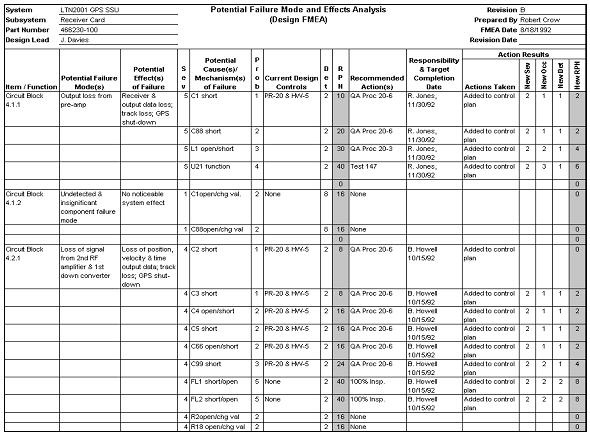
\includegraphics[scale=0.63]{\rootdir/safety/figures/fmea}
  \end{sideways}
  \caption{An FMEA worksheet template}
  \label{fig:safety:fmea-worksheet}
\end{figure}
  

\subsubsection*{Limitations}

Like other safety analysis methods, FMEA has several limitations:

  \begin{itemize}

    \item Frequently, human errors and hostile environments are overlooked.

    \item Because the technique examines individual faults of system  elements taken singly, the combined effects of coexisting  failures are not considered.

    \item If the system is at all complex, the process can be tedious and time consuming.

    \item Failure probabilities can be hard to estimate.

    \item Sometimes FMEA is done only to satisfy the altruistic urge  to ``do safety''. 

  \end{itemize}

FMEA will find and summarise system vulnerability to \emph{single point} failures, and it will require lots of time, money and effort. An important question to ask before undertaking an FMEA is: \emph{how will the results be used?}
  

% LocalWords:  EFCS MTBF lifecycle IEC Therac Mulhouse Habsheim FMGC
% LocalWords:  CommandPoint FADEC pre FMGCs L'affaire Mellor Okecie
% LocalWords:  Kulmbach WoW LGCIU FADECs Mellor's HAZOP PHA EFCSs lp
% LocalWords:  counterfactual Counterfactuals counterfactuals lllllll
% LocalWords:  lll lcccc Operability FMEA HAZOPS HAZard OPerability
% LocalWords:  guidewords guideword Zhangjin llllllllll Backflow llp
% LocalWords:  Accel erate struct voltometer severities lifecycles
% LocalWords:  radia
